Стандарт PDF начиная с версии 1.3, введенный компанией Adobe \cite{adobe}, предусматривает возможность использования интерактивных элементов внутри документа, в том числе созданных с использованием сценарного языка программирования JavaScript. Такую возможность часто используют для сокрытия какой-либо информации или дополнительного функционала, которые при беглом просмотре могут быть незаметны. 

Исходя из этого встал вопрос о поиске таких «подозрительных» файлов в исследуемой системе.

Задание: написать плагин, который будет находить PDF документы со встроенными JavaScript сценариями (рис.~\ref{lob_8:lob_8}).

\begin{figure}[h!]
\center{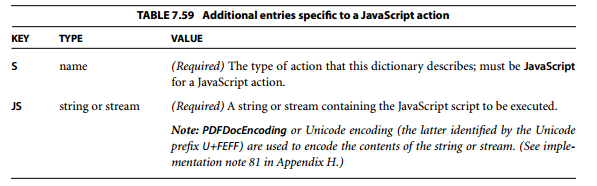
\includegraphics[width=1\linewidth]{lob_8}}
\caption{Вырезка из стандарта PDF 1.3}
\label{lob_8:lob_8}
\end{figure}

Согласно этому стандарту, все JavaScript сценарии обрамляются обязательным ключом <<JS>>, поэтому задача сводится к обнаружению этого ключа в заголовочном блоке PDF документа. Для этого был реализован алгоритм (представлен на рисунке~\ref{lob_9:lob_9}). Результат работы плагина можно увидеть на рисунке~\ref{lob_10:lob_10}.

\begin{figure}[h!]
\center{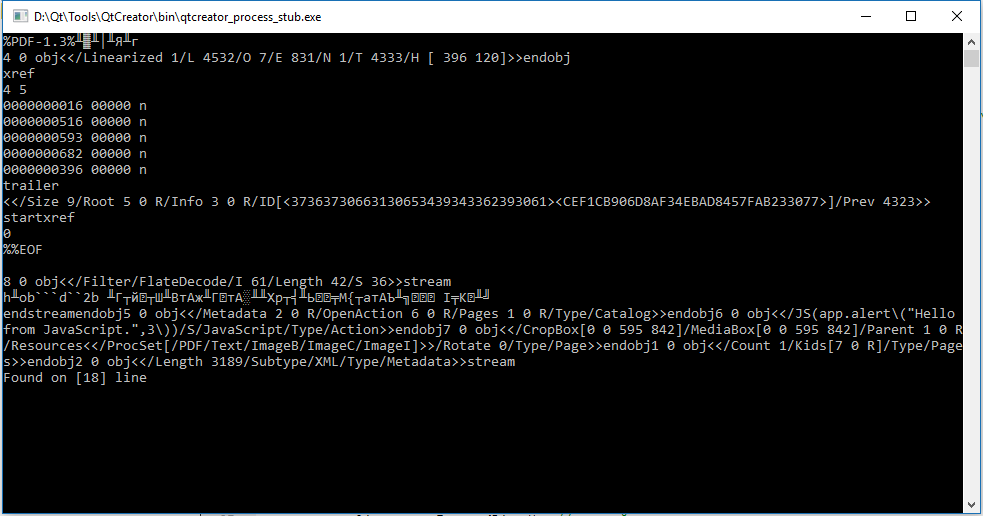
\includegraphics[width=0.8\linewidth]{lob_10}}
\caption{Результат работы плагина}
\label{lob_10:lob_10}
\end{figure}

\begin{figure}[h!]
\center{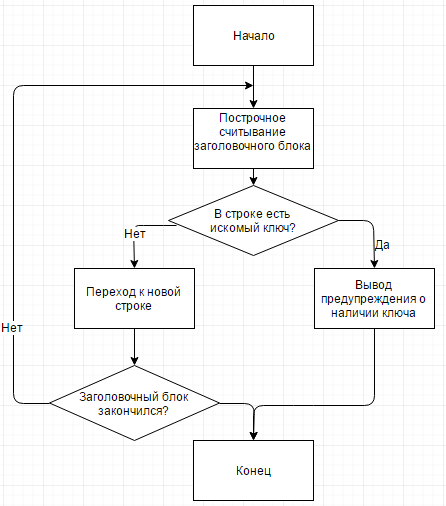
\includegraphics[width=0.8\linewidth]{lob_9}}
\caption{Алгоритм поиска JavaScript в PDF}
\label{lob_9:lob_9}
\end{figure}

\clearpage
